% This is samplepaper.tex, a sample chapter demonstrating the
% LLNCS macro package for Springer Computer Science proceedings;
% Version 2.20 of 2017/10/04
%
\documentclass[runningheads]{llncs}
%
\usepackage{graphicx}
\usepackage{url}
\usepackage{booktabs}
\usepackage{tabularx}
\usepackage[table]{xcolor}
\usepackage{tikz}
\usetikzlibrary{arrows.meta,fit,positioning,shapes.geometric}
\raggedbottom
\setlength{\emergencystretch}{3em}
% Used for displaying a sample figure. If possible, figure files should
% be included in EPS format.
%
% If you use the hyperref package, please uncomment the following line
% to display URLs in blue roman font according to Springer's eBook style:
% \renewcommand\UrlFont{\color{blue}\rmfamily}

\begin{document}
%
\title{An Extensible Activity Architecture for Cross-Platform Music-Learning Applications}
%
\titlerunning{An Extensible Activity Architecture for Music Learning}
% If the paper title is too long for the running head, you can set
% an abbreviated paper title here
%
\author{Anonymous Author(s)}
%
\authorrunning{Anonymous Author(s)}
% First names are abbreviated in the running head.
% If there are more than two authors, 'et al.' is used.
%
\institute{Affiliation withheld for double-blind review}
%
\maketitle              % typeset the header of the contribution
%
\begin{abstract}
Music-learning applications are frequently organized around one educational
activity, making later pedagogical extensions expensive and difficult to
validate. We present an extensible activity architecture for a hybrid
web, Android, and iOS music-learning application. The architecture separates a
bounded shared lifecycle and reusable capabilities---clock, audio, pitch input,
notation, instrument definitions, and persistence---from activity-specific
pedagogical logic. We instantiate it with two functionally and temporally
contrasting activities. Prepare--listen--play is a fixed-cycle, clock-driven
fingering activity; target intonation is driven by pitch estimates, stability,
timeouts, and learner commands relative to an explicit written and sounding
pitch target. Deterministic evaluation comprises 98 automated tests, lifecycle
and dependency-boundary checks, typed instrument and asset audits, and
web/Android/iOS build verification. A post-migration change-surface analysis
shows that the second activity added a separate controller and evaluator,
required a six-line shared contract extension, introduced no
activity-specific branches in the shared core, and left the first activity
controller byte-for-byte unchanged. These results demonstrate that the bounded
lifecycle and capability architecture can support contrasting music-learning
activities with localized modification while retaining cross-platform
maintainability.

\keywords{Music Education Technology \and Software Architecture \and
Extensibility \and Cross-Platform Applications \and Pitch Feedback \and
Open-Source Software.}
\end{abstract}
%
%
%
\section{Introduction}\label{sec:introduction}

As educational technology continues to evolve, its potential to improve learning outcomes in various fields, including music education, has become increasingly apparent. Several studies have explored the role of technology in facilitating both vocal and instrumental training~\cite{Webster12,Bauer20,Fiuza22}. These advancements highlight the transformative power of digital tools in enriching traditional music pedagogy.

One of the key benefits of integrating technology into music education is its capacity to support the development of sensorimotor schemes~\cite{Leman17}. These schemes enable musicians to anticipate the sensory outcomes of their actions, ultimately refining fine motor control. Educational technology, when thoughtfully designed, can play a critical role in reinforcing these schemes by providing real-time feedback and structured practice environments. This facilitates more efficient skill acquisition and allows students to focus on the creative and expressive dimensions of music-making, enhancing both the learning process and artistic outcomes.

Educational technologies have often been designed with a teacher-centered approach, where students are relatively passive recipients of instruction. Studies, such as those by Welch et al.~\cite{Welch05} and Robine et al.\cite{Robine07}, highlight the use of visualization and real-time feedback systems to enrich vocal pedagogy, providing teachers with tools to deliver more immediate and frequent feedback during lessons. While these systems enhance the educational experience, they can limit students’ autonomy and opportunities for independent learning.

Recently, the pedagogical discourse in music education has shifted significantly~\cite{Lennon12}. Traditional instrumental and vocal instruction approaches focused on demonstrating technical skills and providing extensive verbal instruction, modeling, and feedback, while dedicating relatively little time to active student engagement in playing or singing during lessons~\cite{Crocco21}, thereby limiting opportunities to foster student autonomy and lifelong learning skills~\cite{Gaunt08}.
In contrast, contemporary pedagogical trends increasingly prioritize learner-driven approaches that emphasize the learning processes over musical products. This shift encourages strategies such as self-assessment and autonomous error correction~\cite{Harrison14}. New trends promote student independence and incorporate peer learning methods, thus encouraging students’ active participation in the educational process.

Despite the willingness of students and professionals to embrace technology in music education~\cite{Waddell19}, the available technology options have yet to address the full spectrum of music technical skills.
Widely adopted music educational tools are based on the metronome and tuner, due to their ability to make abstract musical concepts (i.e., rhythm and pitch) immediately accessible in real time~\cite{Acquilino22}. Without these tools, teaching such concepts would be significantly more challenging. These technologies facilitate a clearer understanding of technical concepts and musical goals through an audiovisual approach, enhancing the quality of students’ practice sessions and promoting self-regulated learning.
However, beyond rhythm and intonation, there are other technical musical skills that musicians must develop to effectively express their musical ideas, which have received comparatively less attention in terms of dedicated technological solutions.
These skills may be broadly applicable across various categories of musical instruments (e.g., dynamics) or may be more instrument-specific (e.g., articulation). This gap between musical skills documented in the pedagogical literature and available educational technology underscores the opportunity for technology to play a more significant role in music education.

A few studies have developed interactive, multimodal systems that serve as real-time feedback mechanisms, monitoring performance parameters such as pitch, sound quality, and movement across various musical contexts~\cite{Romani15,Bandiera16,Brennan16,Blanco21,AcquilinoSMAC}. However, the widespread adoption of these technologies is often hindered by their reliance on complex PC software, overcomplicated interfaces, and costly hardware setups~\cite{Acquilino22}. These limitations highlight the need for more accessible and user-friendly technological solutions.

In recent years, mobile devices such as smartphones and tablets offer new possibilities for educational approaches and applications in music learning~\cite{Nijs14}.
Mobile apps provide flexible, portable, and ubiquitous solutions, enabling learners to practice anywhere. These platforms also deliver real-time feedback and adapt content to the learner's skill level through user-friendly interfaces, making them valuable tools for enhancing learning experiences~\cite{Paule17,Shi23}.

Despite these advantages, developing mobile applications requires advanced programming skills that might not be part of the expertise of those working in music education technology research. This presents a significant barrier for academic researchers and educators, who are then compelled to seek external support-which is often difficult to obtain-or to settle for simpler, potentially less effective alternatives. These obstacles hinder the development of mobile solutions that could contribute to bridging the gap in empirical research needed to fully understand the impact of technology on music education, as highlighted by Leman and Nijs~\cite{Leman17}.

The software challenge is related but distinct. Music-learning applications
are commonly built around a single practice protocol: timing, audio, pitch
analysis, persistence, and view transitions become interwoven with the
pedagogical sequence that motivated the first release. Adding a second
activity can therefore require restructuring the application instead of
implementing only the new learning logic. A useful architecture must preserve
activity-specific pedagogy while making resource ownership, termination, and
musical targets consistent across activities.

Software-architecture research treats modifiability as a quality attribute
shaped by architectural decisions rather than by component count
alone~\cite{Bass21}. Parnas's classic decomposition criterion similarly places
decisions likely to change behind module interfaces so that change need not
propagate through the system~\cite{Parnas72}. These principles motivate the
separation used here. Our evaluation makes them concrete through a second
activity and a repository-history change scenario~\cite{Bengtsson04} rather than inferring
extensibility from the presence of reusable interface components.

This paper presents an extensible activity architecture extracted from a
pedagogically grounded hybrid application for web, Android, and iOS. It
addresses the research question: \emph{Can a bounded shared lifecycle and
capability architecture support music-learning activities with contrasting
temporal and feedback semantics while localizing change and preserving the
first activity?} We investigate the question through a longitudinal
architecture reconstruction and a second vertical-slice implementation rather
than through an educational-effectiveness study.

The paper makes four contributions:
\begin{enumerate}
  \item a typed, bounded activity lifecycle that separates shared resource
  capabilities from activity-specific pedagogical state;
  \item two complete instantiations---a clock-driven prepare--listen--play
  activity and an event-driven target-intonation activity---on one
  cross-platform application;
  \item a deterministic evaluation of behavior, pitch-target semantics,
  resource ownership, and platform composition; and
  \item repository-history and change-surface evidence showing that the second
  activity required minimal shared evolution and no modification to the first
  activity controller.
\end{enumerate}
The source artifact and build instructions are supplied anonymously for
review.\footnote{The archival artifact URL will be inserted in the submission
version; the public repository URL will be restored after double-blind
review.} Sections~\ref{sec:rationale} and~\ref{sec:during} retain the
pedagogical rationale that produced the two activity requirements.
Section~\ref{sec:architecture} describes the architecture;
Section~\ref{sec:instantiations} compares its instantiations; and
Sections~\ref{sec:evaluation}--\ref{sec:limitations} present the technical
evaluation, interpretation, and limitations.


\section{Pedagogical Rationale}
\label{sec:rationale}

This section presents the pedagogical rationale underlying the design choices of the proposed mobile application. Educational theory and best practices significantly informed how each feature of the app was conceptualized and implemented. Specifically, principles related to building upon existing knowledge, scaffolding, errorless learning, combined practice, auditory imagery, multi-sensory engagement, and imitation guided the app’s instructional structure and user interface. By clearly establishing the theoretical basis first, we clarify the alignment between educational principles and design choices, which are subsequently detailed in Section~\ref{sec:during}.


\subsection{Building upon Existing Knowledge}
\label{sec:starting_known}

Current pedagogical insights emphasize the importance of constructing new knowledge based on what learners already know~\cite{Maton09}. Beginners typically find certain notes or pitch ranges easier to perform, influenced by individual factors such as body characteristics or equipment. Recognizing this principle, the app explicitly allows users to set their preferred pitch range and tempo when initiating an exercise. This customization ensures that learners start from a comfortable and achievable level tailored to their current technical abilities, facilitating more effective and accessible skill acquisition.


\subsection{Scaffolding from Known to Unknown}
\label{sec:scaffolding}

An effective educational approach involves gradually increasing complexity by setting progressively challenging goals that build on previously acquired knowledge. This ensures each new learning step remains intriguing and achievable~\cite{Booth09}. According to Steenstrup~\cite{Steen17}, breaking down large tasks into smaller, manageable components guides learners toward mastery of complex musical skills. Reflecting this scaffolding approach, the app structures exercises in manageable units, allowing users to define their own pitch range and tempo when initiating an exercise and then progressively expand the range or increase the tempo as their skills develop. In the prepare--listen--play activity, intentionally withholding automated corrective feedback preserves space for independent comparison with an explicit auditory model~\cite{Guadagnoli01}; the target-intonation activity instead isolates intonation and makes its feedback criterion explicit. These activity-specific choices illustrate why pedagogical policy remains outside the shared lifecycle.


\subsection{Errorless Practice}
\label{sec:errorless_practice}

Errorless practice involves structuring learning tasks to minimize opportunities for mistakes, thereby enhancing confidence, security and motivation, particularly during early stages of skill acquisition. In motor-learning research, practice conditions that initially reduce task difficulty or complexity are recognized to facilitate skill acquisition by optimizing the balance between challenge and achievable performance~\cite{Guadagnoli04}. Similarly, research in instrumental practice suggests that careful, error-minimizing approaches-such as slow, deliberate initial practice-can significantly boost learners’ confidence and sense of accomplishment, creating a supportive and motivating learning environment~\cite{Allingham23}. Reflecting these principles, the app’s customizable design allows learners to carefully select manageable pitch ranges and tempos, incrementally adjusting these parameters as their proficiency increases. This structured approach helps beginners, in particular, to experience frequent success, build confidence and maintain engagement, supporting sustained learning and performance development.


\subsection{Combined Practice}

Combined practice in music involves the simultaneous use of multiple practice modalities, such as physical practice, mental rehearsal, auditory imagery and singing, to enrich the overall learning experience. Such an approach has been shown to be as effective as extensive physical practice alone in improving technical skills, pitch accuracy and musical expression~\cite{Steen21}. Alternating practice modalities can also reduce physical strain, mitigating the risk of overuse injuries~\cite{Hagglund96}, and has been demonstrated to enhance long-term retention more effectively than traditional blocked practice~\cite{Vera08}.

Reflecting these principles, the proposed app explicitly integrates physical performance with auditory imagery by structuring exercises around active listening immediately followed by playing. While singing is not explicitly required in the current app version, its design naturally accommodates creative integration of additional modalities, such as singing or mental rehearsal, during practice sessions. For instance, learners might sing along with the professional recording during the listening measure before playing, thus reinforcing the auditory-motor connection. Future iterations of the software could further embed combined practice principles by incorporating explicit instructions and integrated feedback for singing or other multimodal strategies, providing users with comprehensive support for diverse, effective and expressive musical practice.


\section{Pedagogical Requirements and Activity Design}
\label{sec:during}

The proposed app’s design directly translates the pedagogical principles discussed above into practical features aimed at effectively supporting musical learning, with an initial focus on fingering techniques for trumpet, clarinet and oboe.


\subsection{Support Correct Fingering Technique}
\label{sec:fingering}

Correct fingering technique requires learners to form accurate associations between musical notation, corresponding motor actions (i.e., finger positioning), and their auditory outcomes. Effective pedagogical practices for teaching fingering could emphasize integrating these visual, motor and auditory cues into a coherent learning experience.
For instance, technologies that explicitly link visual representations of musical notes, note names, and fingerings with auditory examples can significantly enhance learners’ ability to internalize these relationships. Such multimodal integration would strengthen sensorimotor mappings, facilitating learners to internalize technical gestures and develop auditory anticipation skills.

The need for such structured support is especially evident in instruments where the same fingering can yield multiple possible pitches. For example, on the trumpet a single valve position may correspond to several notes in the harmonic series, depending on the player’s embouchure and airflow. This can be confusing for beginners, who may struggle to determine which of the possible pitches is intended for a given notation. In this context, hearing a reference pitch before attempting to play would be particularly important, as it clearly establishes the expected outcome and supports the development of accurate pitch-targeting and auditory imagery.

Several technologies have been proposed to assist with fingering acquisition, including visual aids projected onto screens~\cite{Yin05}, robotic tutors~\cite{Bagga19}, and augmented instruments~\cite{Li22}. However, these tools often focus on overall performance assessment. They tend to prioritize real-time feedback on pitch accuracy and timing rather than supporting the isolated acquisition of specific technical skills such as fingering. As argued by Acquilino and Scavone~\cite{Acquilino22}, this performance-oriented focus may limit pedagogical effectiveness for beginners who are still developing foundational sensorimotor associations.

To better support skill development, instructional activities should provide opportunities for focused, repetitive practice of individual components outside the context of performance. Exercises structured around short, repeated tasks---such as producing a single tone---enable learners to concentrate on the association between finger position, pitch and notation, without the additional cognitive load of timing or sequencing. While such repetition may resemble blocked practice, the structure can also be adapted to interleaved or random practice strategies, as discussed by Stambaugh~\cite{Stambaugh11} and Carter and Grahn~\cite{Carter16}, thereby aligning with current best practices in motor learning. The app developed in this study exemplifies this approach by integrating these elements into its design, as described in Section~\ref{sec:technology}.

\subsection{Facilitation of Auditory Imagery}

Auditory imagery involves cultivating a clear mental representation of sounds prior to physical performance and is an important skill for supporting accurate sound production and expressive musical performance. To effectively cultivate auditory imagery, learners benefit from structured opportunities to internalize accurate pitch and timbral qualities through active listening prior to playing~\cite{Brown13}.

Integrating professional-quality reference tones, such as recordings performed by skilled musicians, could significantly support the development of auditory imagery by providing learners with clear auditory models. Consistent exposure to these high-quality sounds enables students to form robust mental representations, improving their auditory and motor accuracy during subsequent physical performance. Additionally, because auditory imagery encompasses not only pitch but also timbral characteristics~\cite{Halpern04}, recordings from professional musicians, rather than synthesized tones, offer the advantage of richer and more realistic auditory cues.

A pedagogically effective approach may follow a structured sequence. Learners first mentally and physically prepare the required motor action, then actively listen to a high-quality reference recording, and subsequently execute the musical action themselves. Such a design integrates auditory imagery with motor imagery, creating anticipatory mental representations of musical actions and engaging the auditory-motor loop, which Steenstrup~\cite{Steen23} frames as a pedagogical model linking sound perception with motor execution. Neuroscientific research underscores the value of this connection, highlighting the auditory cortex’s role in facilitating precise motor responses in musicians~\cite{Zatorre05,Gates21}.

The app described in Section~\ref{sec:technology} explicitly incorporates this structured auditory imagery training, demonstrating a practical implementation of these pedagogical principles.


\subsection{Multi-sensory Engagement}

Playing a musical instrument inherently engages multiple senses. Generally, musicians interact with the instrument through touch, feel vibrations on the instrument and their body, perceive the resulting sound, and may move in space while playing. This multi-sensory engagement is crucial for developing a comprehensive understanding and mastery of the instrument~\cite{Karakaş24}.

An effective pedagogical strategy could leverage this approach by integrating visual, auditory, tactile and kinesthetic feedback. Visual aids illustrating correct fingerings can guide students in associating notes with specific finger positions, reinforcing tactile memory essential for developing muscle memory~\cite{Schmidt20}. Auditory cues, such as provided reference sounds, would further support learners in forming clear mental representations of target sounds. Additionally, kinesthetic feedback, such as feeling vibrations during actual playing, is integral to refining technique and embouchure through an enhanced physical awareness of sound production~\cite{Kohut85}.

An exercise that alternates periods of preparation, listening and performance could facilitate the integration of multiple sensory modalities. During the preparation phase, learners mentally anticipate the required motor actions by engaging visual and tactile modalities; for example, by setting up fingerings or positioning their hands according to the task. In the listening phase, they actively engage their auditory perception by internalizing a high-quality reference sound. Finally, in the performance phase, tactile, auditory and kinesthetic senses are simultaneously engaged in the execution of the musical gesture. Such multi-sensory engagement aligns closely with McCoy’s model of singing instruction, derived from the VARK framework, which distinguishes auditory, visual, kinesthetic and intellectual modalities~\cite{McCoy04,Fleming92}. The design therefore provides multiple representations of the same task without assuming that learners possess fixed learning styles; its educational effect remains an empirical question~\cite{Fleming06}.


\subsection{Imitation}
\label{sec:Imitation}

The previously discussed pedagogical principles share a common foundation in imitation, a fundamental mechanism of human learning~\cite{Rizzolatti04}. Employing visual references along with auditory models can effectively stimulate imitation, thereby enhancing motor and auditory skill acquisition, progressively making the achievement of the musical goal more immediate and transparent, as discussed by Nijs et al.~\cite{Nijs13}.

Furthermore, for instrument categories where timbre plays a central role in guiding performance, providing professional-quality recordings rather than synthesized sounds may offer important pedagogical advantages. Research has shown that timbre quality can influence sound production efficiency in instruments like the trumpet~\cite{AcquilinoISMIR}, building on pedagogical insights that efficiently produced tones are perceived as rich and rounded, while less efficient production tends to result in a shrill or strained quality~\cite{Jacobs06,Steen07}. Introducing music learners to high-quality recorded models could encourage imitation of these efficient production strategies, supporting the development of more refined and expressive performance outcomes.


% The following legacy design, anticipated-outcome, and component-catalogue
% sections are retained in the source history for traceability but are excluded
% from the revised architectural paper.
\iffalse
\section{Application Design and Interface}\label{sec:legacy-technology}

An educational interface has been developed to facilitate learners in acquiring correct instrumental fingering technique by associating visual, auditory and motor cues. As an initial implementation, the interface supports trumpet, clarinet and oboe fingering, assisting learners in internalizing the relationship between musical notation on the staff, the corresponding note names, the required fingering combinations and produced pitch. Screenshots of the main interface are shown in Figure~\ref{fig:Interfaces}a for trumpet and in Figure~\ref{fig:Interfaces}b for clarinet.

\begin{figure*}[t]
\centering
\begin{minipage}[b]{0.235\textwidth}
    \centering
    \fbox{\includegraphics[width=\dimexpr\linewidth-2\fboxsep-2\fboxrule\relax]{BJET1.pdf}}
    \par\smallskip
    \small (a)
\end{minipage}
\hspace{0.01\textwidth}
\begin{minipage}[b]{0.235\textwidth}
    \centering
    \fbox{\includegraphics[width=\dimexpr\linewidth-2\fboxsep-2\fboxrule\relax]{BJET4.pdf}}
    \par\smallskip
    \small (b)
\end{minipage}
\hspace{0.01\textwidth}
\begin{minipage}[b]{0.235\textwidth}
    \centering
    \fbox{\includegraphics[width=\dimexpr\linewidth-2\fboxsep-2\fboxrule\relax]{BJET2.pdf}}
    \par\smallskip
    \small (c)
\end{minipage}
\hspace{0.01\textwidth}
\begin{minipage}[b]{0.235\textwidth}
    \centering
    \fbox{\includegraphics[width=\dimexpr\linewidth-2\fboxsep-2\fboxrule\relax]{BJET3.pdf}}
    \par\smallskip
    \small (d)
\end{minipage}
\caption{(a) Interface with trumpet fingering display. (b) Interface with clarinet fingering display. (c) Options menu. (d) Interface with chromatic tuner.}
\label{fig:Interfaces}
\end{figure*}

The interface enables learners to input practice parameters, such as the metronome value (ranging from 40 to 180 beats per minute), and to define the lowest and highest notes within the typical range of the supported instruments: trumpet [E3--B$\flat$5], clarinet [D3--B$\flat$6] and oboe [B3--G$\sharp$6]. Once configured, pressing the Start button generates a sequence of three measures in 4/4 time signature, displayed in standard Western music notation and accompanied by metronome clicks marking quarter notes at the specified tempo.
The app randomly selects a note within the defined range and displays it in the second and third measures of the score. \textbf{Measure 1} functions as a rest period, giving learners time to visually and tactilely prepare the appropriate fingering for the upcoming note. \textbf{Measure 2} presents a high-quality audio recording of the target pitch, allowing learners to internalize its auditory features. \textbf{Measure 3} prompts the learner to physically play the note, integrating prepared motor actions and auditory expectations. After completing this three-measure sequence, the app randomly selects a new note within the specified range and generates a new three-measure cycle, continuing this loop until the learner taps the Stop button. For additional clarity, the name of the displayed note also appears below the score, and can be shown either in letter notation (C, D, E, …) or in solfège (Do, Re, Mi, …), according to the learner’s preference.

In the top-right corner of the interface, an image of the corresponding fingering to play the displayed note is shown. For the trumpet, this also indicates whether the third-valve slide extension is necessary (e.g., for C$\sharp$4 or D4). Currently, one common fingering is displayed for notes that allow multiple alternatives, although additional fingering options may be incorporated in future app iterations to deepen technical knowledge.

To further guide learners through the exercise, a traffic-light-inspired visual cue system is prominently displayed: red corresponds to rest, yellow to listening and green to active playing. Each color and action is dynamically highlighted in real time during its respective measure, helping users follow the exercise sequence intuitively. In addition, the interface clearly indicates the current beat (1, 2, 3, 4), synchronized with audible metronome clicks.

Supplementary options accessible through a toggle menu (Figure~\ref{fig:Interfaces}c) allow additional customization to support varied learning goals. Here, learners can select the instrument from a drop-down menu. They may also enable a chromatic tuner in place of the fingering image (Figure \ref{fig:Interfaces}d), allowing them to focus on pitch accuracy once they are familiar with the correct fingerings, thus transitioning from note identification to intonation refinement. Other available options include expanding the pitch selection to include accidentals (sharps and flats); if this toggle is not selected, the app selects notes exclusively from the C major scale. Learners can further choose their preferred note nomenclature, selecting either letter notation or solfège. Finally, they may activate random dynamic markings: \textit{piano}, \textit{mezzo-forte}, \textit{forte}. When dynamics are enabled, the selected marking is displayed below the score and the loudness of the reference recording is automatically adjusted to match it, fostering the development of dynamic control.

The application is developed as a cross-platform mobile app compatible with Android and iOS devices, and is also available via web browsers. It is freely accessible through Google Play, the iOS App Store\footnote{To maintain anonymity, the links will be added in the camera-ready manuscript.}, and a dedicated web platform\footnote{\url{https://lobster-app-n5bs2.ondigitalocean.app/home/exercise}}.

The exercise is grounded in a fundamental learning model framework, which provides the flexibility and motor adjustment necessary for facilitating the prosthesis-dialogue modes of instrumental interaction~\cite{Leman17}. The execution of this exercise aims to adhere to elements of a cognitive architecture for sensorimotor processing, specifically:

\begin{itemize}
\item Measure 1 - \textit{The motor command}: During the first measure, which is a rest, the learner can observe the note selected by the software and prepare the correct corresponding fingering on the instrument as indicated in the image on the interface. When done repeatedly, this action trains the neural patterns that control finger movements performing a musical action~\cite{Engel12}.

\item Measure 2 - \textit{The expected sensory outcome of the motor command}: In the second measure, the student listens to the sound of the proposed note recorded by a professional musician. This immediate listening before execution helps develop an auditory-motor loop. An fMRI study by Gebel et al.~\cite{Gebel13} involved trained pianists and trumpet players using an MRI-compatible trumpet model without auditory feedback. Unlike pianists, trumpet players showed a specific co-activation increase in the left primary sensorimotor cortex, particularly in the regions associated with lip movements, the trunk, the right cerebellar hemisphere, and the left primary auditory cortex. As noted by Steenstrup et al.~\cite{Steen21}, this indicates that auditory activity influences motor activity in musicians.

\item Measure 3 - \textit{The real sensory outcome}: In this measure, the learner plays the note and perceives the actual outcome of the musical action. They experience the intended sensory feedback, facilitated by the technology in a manner that is both transparent and mentally unobtrusive.
\end{itemize}

The structured, iterative nature of the exercise is supported by a modular technical architecture designed to clearly separate the interface, logic and data handling components. Figure~\ref{fig:app_architecture} illustrates this architecture, highlighting key services and interactions. A more detailed technical description of the app components and their implementation is provided in Appendix~\ref{sec:repo}.

\begin{figure*}[t]
    \centering
    \includegraphics[width=0.8\textwidth]{app_architecture.pdf}
    \caption{App architecture, showing separated layers (Client Interface, RxJS-based Application Services, and Firebase Data Layer) and labeled flows such as beat ticks and reference-note playback, pitch analysis, and performance logging.}
    \label{fig:app_architecture}
\end{figure*}

This architecture enables a responsive web and mobile interface, allowing learners to engage in self-paced practice across different devices and environments. The following section discusses the anticipated educational outcomes of this design and reflects on its broader implications for music learning and practice.


\section{Anticipated Pedagogical Outcomes and Discussion}
\label{sec:results}

Having outlined the design features and interface structure of the application, this section discusses anticipated pedagogical outcomes derived from its use. Tailoring the learning experience to individual needs is essential for effective skill acquisition and progression. A common strategy for learning a musical instrument is to follow practice methods with predefined sequences of increasing difficulty. However, this standardized, one-size-fits-all approach may not suit all learners, as it assumes a uniform starting point and rate of progress~\cite{Steen23}.

This application offers a more inclusive alternative by supporting learner-centered customization. Learners can set their own initial conditions based on their current skill level, thereby enabling gradual progression that adapts to individual needs. Such flexibility challenges the ableist assumptions embedded in traditional pedagogies---which often normalize linear, uniform development---and instead embraces diverse learning trajectories~\cite{Dolmage17,Hehir02}. By allowing learners to self-regulate task complexity and modality (e.g., visual, auditory, kinesthetic), the design promotes equitable access to musical development, aligning with principles of universal design for learning (UDL) and inclusive music education~\cite{Katz13,Jellison15}.

This learner-centered approach, grounded in established pedagogical theories (Sections~\ref{sec:rationale} and \ref{sec:technology}), highlights anticipated educational benefits outlined below.


\subsection{Maintaining the Flow Zone}
\label{sec:flow_zone}

Introducing progressively more challenging and intriguing tasks helps learners improve their technical skills without losing interest. Csikszentmihalyi~\cite{Csikszentmihalyi08} defines the flow zone as a state of mind where a person is fully concentrated and completely immersed in their current activity. This concept emphasizes the importance of assigning exercises of appropriate difficulty to promote optimal learning. Exercises that are too easy can lead to boredom and loss of motivation, while overly difficult tasks may cause tension, bad habits and a sense of panic. Maintaining this state of attention is fundamental in musical practice, as it can be involuntarily captured or deliberately focused, influencing how learners perceive and interact with their instruments, and shaping their skills and understanding through active exploration and practice~\cite{Tullberg22}.


\subsection{Bridging Abstract Concepts and Practical Skills}

Music, due to its abstract nature, can be difficult for learners to grasp and translate into appropriate actions. As Nijs~\cite{Nijs18} discusses, music is often perceived as abstract and disconnected from concrete events, challenging learners to understand and translate it into practical performance actions. Bridging the gap between abstract musical notation and tangible musical execution can help learners internalize these concepts more effectively.

For example, providing visual and auditory cues, such as displaying correct fingerings alongside a reference pitch, can strengthen the association between abstract musical symbols and the corresponding physical actions. Displaying the note name beneath the staff further reinforces this connection by linking symbolic notation to a verbal label that learners can quickly recognize.
Together, these multimodal cues help demystify abstract concepts, enabling students to better understand and perform musical tasks. Similarly, guiding learners in the acquisition of rhythm through metronome beats and reference examples can improve timing and rhythmic accuracy by making these abstract patterns more concrete and easier to follow.


\subsection{Promoting Alternated Practice and Reflection}

The proposed exercise encourages alternated practice and learner reflection. This approach not only helps beginners in playing long tones, but also combines physical practice with observation, an efficient learning strategy. A study by Larssen et al.~\cite{Larssen21} highlights that interleaving observation and practice benefits visuomotor adaptation and motor memory consolidation. They found that observation can effectively replace physical practice if supplied intermittently, providing benefits beyond mere rest periods.

The inclusion of rest and listening measures in the exercise is motivated by these findings. The rest measure, in addition to allowing learners to prepare the appropriate fingering, also serves as reflection time on their previous performance. While the design offers an opportunity for self-reflection and self-correction, it is important to note that young beginners may not yet have fully developed self-reflective abilities~\cite{AdamsWebber99}. For this reason, instructor or parental guidance may be necessary to support younger learners in evaluating whether they have played the correct note, a process facilitated by the app’s provision of an explicit auditory model.

One reason for not including immediate feedback on note performance is to encourage learners' reflection on their actions. Assuming the goal of the exercise is to learn correct fingering and produce the indicated note (without focusing on intonation at this stage), the interface provides all necessary information, including the corresponding fingering and a realistic reference pitch. This should enable students to discern whether they played the correct note, fostering what is known in motor learning literature as internal reference-of-correctness~\cite{Maas08}.

If the desired sound is not produced, corrective feedback highlighting the error could distract the learner with negative reinforcement. Instead, the current design offers an opportunity for self-reflection and self-correction. As philosopher John Dewey stated, ``\textit{we do not learn from experience... we learn from reflecting on experience}"~\cite{Dewey38}. This emphasis on reflection aligns with studies indicating that alternating physical practice of a new skill with short rest intervals (even for just a few seconds) leads to performance improvements during these brief rest periods, known as \textit{micro-offline gains}~\cite{Bonstrup20}. Personal reflection enables learners to produce the suggested note and internalize the motor and auditory process, bypassing the typical ambiguity of the interpersonal feedback process between teacher and learner~\cite{Welch05}.

Once learners have internalized the basic fingering through self-reflection, they can choose to activate the chromatic tuner option, which replaces the fingering image and provides real-time feedback on pitch and intonation. This functionality supports the transition from note identification to intonation refinement while allowing learners to focus on one technical aspect at a time and avoid cognitive overload. Additionally, the exercise could be adapted to extend the measures of rest, listening and playing based on the student's needs, providing more time for learners to experience the musical action and reflect on it.

By combining these pedagogical principles, the developed interface offers a robust framework for learning fingering technique. The current software's ability to flexibly adjust different difficulty levels should help maintain learners within the \textit{flow zone}, fostering continuous improvement and engagement. Also, it provides both learners and educators with a personalized and engaging approach that supports the learner's progression from known to unknown, in small, achievable steps.

% The present study focuses specifically on the rationale, theoretical foundations and technical design of the developed application. Empirical validation and usability studies involving trumpet learners have been conducted and will be reported\footnote{The study involving participants is not included here primarily due to the 6000-word limit for this publication.}.

\section{Future Directions}
\label{sec:Suggestions_for_future_studies}

The application presented in this study is a work in progress that offers significant potential for future developments. Leveraging open-source practices, we aim to build a collaborative community of researchers, educators and developers to combine, adapt and expand its modular components, fostering innovation in music educational technology. The source code of the app is available in a public GitHub repository. The design of the app is modular and built around the concept of reusable components (see Appendix \ref{sec:repo}). While creating entirely new components still requires substantial coding expertise, this architecture lowers barriers for adaptation and prototyping, facilitating the development of sophisticated tools and accelerating research in fields such as pedagogical design, interactive user interfaces for music education and real-time audio analysis.

This approach functions both as a conceptual (pedagogical) framework and as a modular software (GUI) infrastructure, allowing educators and researchers to build new applications that rest on robust pedagogical foundations while taking advantage of flexible code components. Future developments could expand this synergy to address a broader range of musical skills that are crucial for expressive performance but often lack dedicated technological support. Music education methods for wind instruments, for example, highlight the importance of mastering fundamental aspects such as articulation, attack, breathing, fingering, intonation, rhythm, tone quality and vibrato~\cite{Arban82,Westphal90,Weisberg07}. Yet, many of these remain underexplored in available mobile edTech solutions~\cite{Acquilino22}. By leveraging the hardware capabilities of modern mobile devices (e.g., displays, loudspeakers, microphones), future studies could create new components offering real-time visualization and feedback on these critical skills. The proposed repository offers a flexible framework that can help bridge this gap, gradually expanding into a comprehensive platform for both technical and artistic development.

Although the presented app has so far been developed with a focus on wind instruments and Western music notation, its design allows straightforward extension to other musical instruments and traditions. Future studies could explore its adaptation to diverse pedagogical contexts, embedding alternative notations---including culturally specific systems and formats designed to enhance accessibility---and incorporating feedback mechanisms suited to different instrumental techniques. By supporting a wider variety of musical practices and learning needs, the repository has the potential to become a truly inclusive and adaptable educational tool.

Another promising direction for future research is the integration of gamification elements to increase learner engagement and motivation. Gamification, which involves applying game design principles such as levels, challenges and rewards to educational contexts, has been shown to enhance learning outcomes and enjoyment~\cite{Deterding11}. By transforming repetitive exercises into interactive and rewarding experiences, gamified elements could encourage active participation, sustained motivation and long-term retention of musical skills. Features like progress tracking, customizable difficulty levels and creative challenges could make practice both effective and enjoyable.

Ultimately, the presented application aspires to become more than a tool for technical improvement. Future work and community contributions can evolve it into a holistic educational platform, fostering intrinsic and extrinsic motivation, supporting individualized learning and meeting the needs of diverse musicians. By bridging gaps in existing technologies and expanding its scope, this work has the potential to redefine music education as a more accessible, engaging and meaningful experience for learners worldwide.


\section{Conclusions}
\label{sec:Conclusions}

This paper introduced a novel open-source web technology explicitly designed to embed established pedagogical principles into the development of accessible music learning tools. By foregrounding foundational educational theories, the study demonstrates a concrete application of these concepts through the development of a multimodal mobile app supporting critical technical and auditory skills.
Central design elements, including dynamic audiovisual feedback, structured practice sequencing and learner-driven customization, illustrate how abstract pedagogical concepts can be successfully operationalized to foster individualized and reflective musical practice.

The modular and open-source code framework developed for this project reduces barriers for educators and researchers, making it easier to create and adapt robust educational tools without requiring advanced programming expertise for basic modifications. This approach not only addresses critical gaps in current educational technologies for music but also provides a flexible and extensible foundation adaptable across instruments, musical traditions and learning contexts.

Anticipated outcomes of this educational design include improved learner autonomy, sustained engagement through appropriately calibrated challenges (the flow zone) and enhanced translation of abstract musical concepts into concrete motor skills. By explicitly linking theoretical foundations with technological design, this paper provides a clear pathway for future empirical studies aimed at systematically evaluating these outcomes.

Future directions highlighted by the study underscore the potential of this modular framework to expand into broader pedagogical contexts, support additional instrumental skills and incorporate motivational features such as gamification. These extensions promise to further enrich the educational experiences and effectiveness of the technology.

Ultimately, by strategically aligning pedagogical theory with open-source technological development, this work contributes a valuable model for future innovations in music education technology, advancing both scholarly research and practical teaching methodologies in the field.


% \begin{table}
% \caption{Table captions should be placed above the
% tables.}\label{tab1}
% \begin{tabular}{|l|l|l|}
% \hline
% Heading level &  Example & Font size and style\\
% \hline
% Title (centered) &  {\Large\bfseries Lecture Notes} & 14 point, bold\\
% 1st-level heading &  {\large\bfseries 1 Introduction} & 12 point, bold\\
% 2nd-level heading & {\bfseries 2.1 Printing Area} & 10 point, bold\\
% 3rd-level heading & {\bfseries Run-in Heading in Bold.} Text follows & 10 point, bold\\
% 4th-level heading & {\itshape Lowest Level Heading.} Text follows & 10 point, italic\\
% \hline
% \end{tabular}
% \end{table}



% \begin{figure}
% \includegraphics[width=\textwidth]{fig1.eps}
% \caption{A figure caption is always placed below the illustration.
% Please note that short captions are centered, while long ones are
% justified by the macro package automatically.} \label{fig1}
% \end{figure}



% For citations of references, we prefer the use of square brackets
% and consecutive numbers. Citations using labels or the author/year
% convention are also acceptable. The following bibliography provides
% a sample reference list with entries for journal
% articles~\cite{ref_article1}, an LNCS chapter~\cite{ref_lncs1}, a
% book~\cite{ref_book1}, proceedings without editors~\cite{ref_proc1},
% and a homepage~\cite{ref_url1}. Multiple citations are grouped
% \cite{ref_article1,ref_lncs1,ref_book1},
% \cite{ref_article1,ref_book1,ref_proc1,ref_url1}.
%
% ---- Bibliography ----
%
% BibTeX users should specify bibliography style 'splncs04'.
% References will then be sorted and formatted in the correct style.
%
% \bibliographystyle{splncs04}
% \bibliography{mybibliography}
%
\appendix
\section{Software Structure}
\label{sec:repo}
\vspace*{12pt}

We present an application designed to provide state-of-the-art solutions for music education, leveraging modern web technologies and reusable components. The app is released under the Affero GPL license\footnote{Available at: \url{https://www.gnu.org/licenses/agpl-3.0.html} (accessed December 14, 2024).} and is built using the \emph{Ionic}\footnote{\textit{Ionic} Framework. Available at: \url{https://ionicframework.com/} (accessed December 14, 2024).} framework and \emph{Angular}\footnote{\textit{Angular} Framework. Available at: \url{https://angular.io/} (accessed December 14, 2024).}. These technologies allow developers to create a hybrid mobile app that can run directly in a browser or be deployed as mobile apps for both iOS and Android devices.
The use of widely adopted web technologies ensures compatibility across platforms, broadens accessibility, and allows more developers to contribute to and customize the codebase effectively.

The source code is organized into a set of modular Angular components and services that provide a flexible basis for creating and adapting educational tools.
These reusable components address music educational elements such as score display, note selection, and audio processing (e.g., playing or recording sound). By combining these building blocks, developers can create more sophisticated features, such as a chromatic tuner or customized audio feedback systems. Each component automatically adapts its interface to changes in input or screen size, ensuring a responsive layout across platforms and devices.
The entire application relies on a service that establishes timing for triggering events. The service uses RxJS\footnote{\textit{RxJS}, a library for reactive programming in JavaScript. Available at: \url{https://rxjs.dev/} (accessed December 14, 2024).} to emit events at intervals defined by the user.

For detailed information on the components and how to use the repository, we invite the reader to refer to the online documentation\footnote{To maintain anonymity, the repository is available as an anonymous Google Drive download. The direct GitHub link will be provided in the camera-ready version of the manuscript.}.

\subsection{Reusable App Components\label{sec:components}}

The following functional components have been designed in the application framework:


\subsubsection{Tempo Selector\label{sec:metronome}}

This component allows users to select the tempo in beats per minute (bpm) in a GUI optimized for mobile devices.


\subsubsection{Note Selector Component}

This component offers an intuitive interface for selecting individual musical notes for a given exercise. The current note is displayed as an image, and tapping it opens a scrollable modal gallery of note images, enabling specific note selection.
This interface supports various clefs (e.g., treble or bass) and can be configured to display subsets of notes (e.g., specific scales like chromatic or C major).


\subsubsection{Score Display Component}

The \textit{Score Display} component renders dynamic and responsive musical scores using VexFlow\footnote{\textit{VexFlow} library for rendering music notation in the browser. Available at: \url{https://github.com/vexflow/vexflow} (accessed December 14, 2024).}. It accepts a score object containing detailed Western music notation elements such as measures, clef, key signature, time signature, dynamics, and notes. It can be fed with predefined scores or generate them on the fly via random or deterministic algorithms, or even AI-based approaches. Parameters like the lowest and highest notes or specific scales are also configurable, enabling a wide range of educational scenarios.


\subsubsection{Fingering Display Component}

The \textit{Fingering Display} component embeds static or vector images within an application’s interface. Taking trumpet as an example, a GUI created with SVG displays a detailed illustration of a trumpet along with interactive buttons. These buttons simulate sliding mechanisms and turn red when activated, visually indicating the corresponding trumpet fingering for the note to be played.
To enable interactivity, visual indicators or feedback can be synchronized with metronome data or performance metrics. This feature allows developers to provide real-time visual feedback on technical aspects of music learning.


\subsubsection{Exercise Guide Component}

This component visually guides users through different phases of the musical exercise: rest, listen, and play. It uses a traffic light representation with red, yellow, and green lights representing each phase, helping users follow a structured flow of activities. By providing clear visual cues, this feature enhances focus and rhythm during practice sessions.


\subsubsection{Audio Output}

The application uses this service to manage the timed playback of sounds. These can be pre-recorded or synthesized sounds managed through the MIDI protocol and allow real-time modulation of musical parameters such as duration and dynamics.


\subsubsection{Audio Input}

The \textit{Audio In} service acquires real-time audio from the device microphone%, sampling at 44.1 kHz by default
. While its simplest use case is straightforward audio recording, the component is designed to serve as a foundation for more advanced sound analysis tools.


\subsubsection{Chromatic Tuner Component}

The \textit{Chromatic Tuner} component uses the \textit{Audio In} service for real-time pitch detection. It implements the pitch-tracking algorithm proposed by McLeod~\cite{McLeod05}, identifies the detected pitch, and compares it to a reference frequency (default equal temperament with A4 = 440 Hz). An interface displays note names, cent deviations, and visually indicates whether the current pitch is in tune, sharp, or flat via an animated SVG pointer. Emoji-based feedback further enhances user engagement, showing ``in tune”, ``slightly off”, or ``out of tune” states. The tuner can function as a standalone feature or be embedded within more comprehensive exercises to provide immediate and precise intonation feedback.


\subsubsection{User Performance Tracking}

This service leverages the \emph{Firebase Realtime Database}\footnote{Google Firebase, \textit{Firebase Realtime Database}. Available at: \url{https://firebase.google.com/} (accessed December 14, 2024).} to log user performance data (e.g., number of errors) alongside multiple usage statistical metrics. An optional user registration system enables personalized tracking while preserving user anonymity. The collected data can inform pedagogical research or guide the development of targeted application features, bridging the gap between industry-grade tracking tools and academic research goals.


\subsection{Project Sustainability}

The long-term sustainability of this open-source initiative is grounded in community engagement and transparent development. The project is hosted publicly and version-controlled, inviting contributions, adaptations and feedback from educators, researchers and developers. Ongoing maintenance is currently led by the author(s) of this manuscript.

This application also represents a component of a broader, structured research and development initiative. Details about this overarching project will be shared in future stages of the review process and in the camera-ready version of this manuscript, as anonymity must be preserved at this time due to the double-blind review.

We view open-source development as both a technical and pedagogical commitment: fostering collaboration, reproducibility and equity in music education technology.



\fi

\section{User-Facing Activities}\label{sec:technology}

The application now exposes two independent activity routes (Fig.~\ref{fig:ui}).
Both begin from an explicit typed instrument and written-note range, but they
organize learner action differently. The prepare--listen--play (PLP) route
supports the original fingering and auditory-imagery design: the learner
prepares a fingering, listens to a recorded reference, and plays during a
metered window. The target-intonation route presents a written target, can play
the corresponding reference tone, and then evaluates incoming pitch relative
to that target. A learner selects either activity without entering a generic
exercise editor; pedagogical configuration remains specific to the selected
activity.

\begin{figure}[t]
\centering
\begin{minipage}[t]{0.46\textwidth}
  \centering
  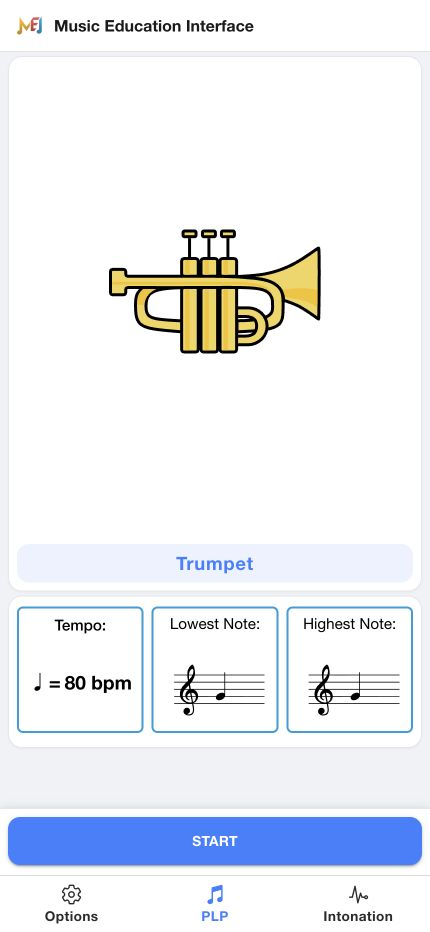
\includegraphics[height=.39\textheight,keepaspectratio]{figures/plp-launch.png}\\[-1mm]
  {\small (a) Prepare--listen--play}
\end{minipage}\hfill
\begin{minipage}[t]{0.46\textwidth}
  \centering
  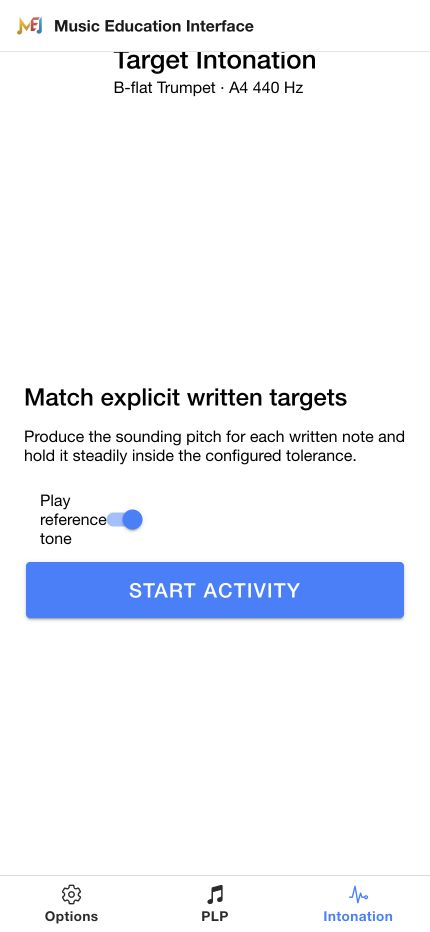
\includegraphics[height=.39\textheight,keepaspectratio]{figures/target-intonation-launch.png}\\[-1mm]
  {\small (b) Target intonation}
\end{minipage}
\caption{Current mobile-responsive entry surfaces for the two activities.
PLP exposes instrument, tempo, and note-range configuration; target intonation
states its explicit-target task and optional reference-tone policy. The shared
tab host switches activities through independent routes and cancels an active
session before supersession.}
\label{fig:ui}
\end{figure}

The two routes embody a deliberate contrast. PLP is clock-driven and
non-gating: pitch feedback, when enabled, does not determine phase progression.
Target intonation is event-driven and gating: progress depends on a valid
estimate for the expected sounding note, an in-tolerance stability window, an
attempt timeout, or a learner command. This contrast is central to the
architectural evaluation because it tests whether one shared lifecycle can
support different time models and feedback policies without absorbing either
activity's pedagogy.

\section{Architecture}\label{sec:architecture}

\subsection{Design Goals}

The reconstruction was guided by four requirements. First, shared code should
define only lifecycle and capabilities common to both activities. Second,
written and sounding pitch must be unambiguous for transposing instruments.
Third, the controller that starts a resource must own its cancellation and
terminal cleanup. Fourth, views should present typed snapshots and dispatch
commands without controlling microphones, clocks, or persistence.

Figure~\ref{fig:architecture} summarizes the resulting dependency direction.
The host admits one active controller through an activity-session service.
Controllers depend on an \texttt{ActivityContext} of narrow ports rather than
browser, mobile, or database APIs. Adapters implement those ports at the
application boundary. Instrument definitions and pitch mathematics form a
typed musical domain shared by both activities, while state transitions remain
inside the two activity modules.

\begin{figure}[t]
\centering
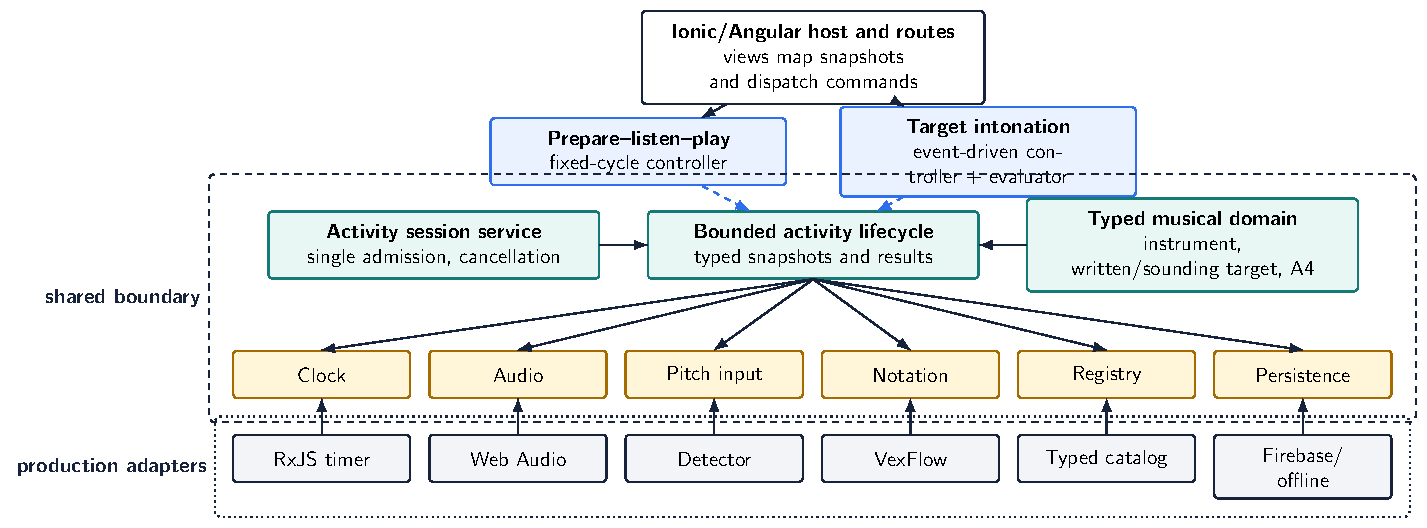
\includegraphics[width=\textwidth]{figures/activity-architecture.pdf}
\caption{Implemented dependency structure. The bounded lifecycle and session
service coordinate activity admission and termination; capability ports expose
clock, audio, pitch input, notation, instrument registry, and persistence.
Activity controllers own pedagogical transitions and depend inward on these
contracts. Platform and service adapters remain outside the controller
boundary.}
\label{fig:architecture}
\end{figure}

\subsection{Bounded Lifecycle and Session Admission}

Every controller implements the same small contract:
\texttt{configure}, \texttt{start}, \texttt{cancel}, \texttt{restart}, and a
snapshot stream. The lifecycle envelope is a discriminated union of
\texttt{idle}, \texttt{starting}, \texttt{running}, \texttt{completed},
\texttt{cancelled}, and \texttt{failed}. Only the \texttt{running} variant
contains activity-specific state. Terminal variants contain a typed result,
which makes completion, cancellation, and failure explicit instead of
overloading a view flag.

\texttt{ActivitySessionService} enforces single admission. Starting a new
controller supersedes the current session; route changes and application
backgrounding use the same cancellation boundary. This central admission rule
prevents two activities from competing for microphone, audio, or persistence
resources while leaving the internal transition model to each controller.

\subsection{Capability Ports and Ownership}

\texttt{ActivityContext} contains clock, audio, pitch-input, notation,
instrument-registry, persistence, and injected-randomness ports. The clock
supports periodic ticks and one-shot deadlines, both with abort signals.
Pitch input exposes timestamped voiced or unvoiced estimates and returns an
acquired session with one release operation. Audio exposes metronome and
target-relative reference playback. Persistence opens and closes a typed
session envelope.

Controllers acquire these capabilities during startup and release them on
completion, learner stop, navigation, supersession, startup failure, or runtime
failure. Terminal entry is guarded, and cancellation is idempotent. This is
important for mobile navigation, where an explicit learner command, route
teardown, and operating-system lifecycle event can occur close together. The
views never connect or disconnect the microphone.

\subsection{Typed Musical Domain}

A \texttt{NoteTarget} binds written spelling, sounding spelling,
instrument transposition, selected reference A4, expected sounding frequency,
notation, fingering/valve representation, and the reference-tone asset.
Expected frequency is computed once:
\[
 f_{\mathrm{target}} = f_{\mathrm{A4}}\,
 2^{(m_{\mathrm{sounding}}-69)/12}.
\]
The registry currently defines B-flat trumpet and B-flat clarinet at
$-2$ semitones and C oboe at zero semitones. It contains 110 typed note
definitions and resolves 189 exact production asset paths. The same target is
passed to notation, playback, and evaluation, avoiding independent
written-to-sounding conversions in views or controllers.

\subsection{Bounded Results and Persistence}

Both activities produce a common result envelope containing the activity and
version identifiers, session identifier, outcome, timestamps, and any
cancellation or failure reason. PLP adds planned/completed cycles, presented
targets, and bounded pitch summaries. Target intonation adds its explicit
configuration and per-attempt outcomes, including time to first valid
estimate, time to stable hold, valid-estimate and wrong-note counts, median
cents, absolute-error percentile, and spread when available. Production
telemetry stores no microphone audio and no full per-frame pitch trace.
Activity-specific persistence dispatch occurs in the Firebase adapter, outside
the shared lifecycle.

\section{Two Architectural Instantiations}\label{sec:instantiations}

\subsection{Clock-Driven Prepare--Listen--Play}

PLP owns the states \texttt{preparing}, \texttt{listening}, and
\texttt{playing}. Each phase has four beats, and the default activity has 12
cycles. The deterministic default trace therefore contains 144 running ticks,
144 metronome commands, and 12 reference-tone commands. Completion occurs
after cycle 12, Play beat 3; no sentinel tick or duplicate terminal playing
state is emitted. Optional pitch estimates are descriptive and cannot advance
or delay the sequence. A learner stop yields a cancelled result and retains
bounded summaries already collected.

\subsection{Event-Driven Target Intonation}

Target intonation owns the states \texttt{presenting-target},
\texttt{awaiting-signal}, \texttt{tracking}, and
\texttt{attempt-result}, inside the shared running lifecycle
(Fig.~\ref{fig:lifecycles}). Its commands are
\texttt{retry-attempt}, \texttt{next-target}, \texttt{skip-target}, and
\texttt{stop}. Optional reference playback occurs while the target is
presented. Pitch acquisition then drives feedback and stable-hold progress;
one-shot timers drive presentation and attempt deadlines. The controller can
retry or skip according to the configured attempt policy and completes after
the configured number of targets.

\begin{figure}[t]
\centering
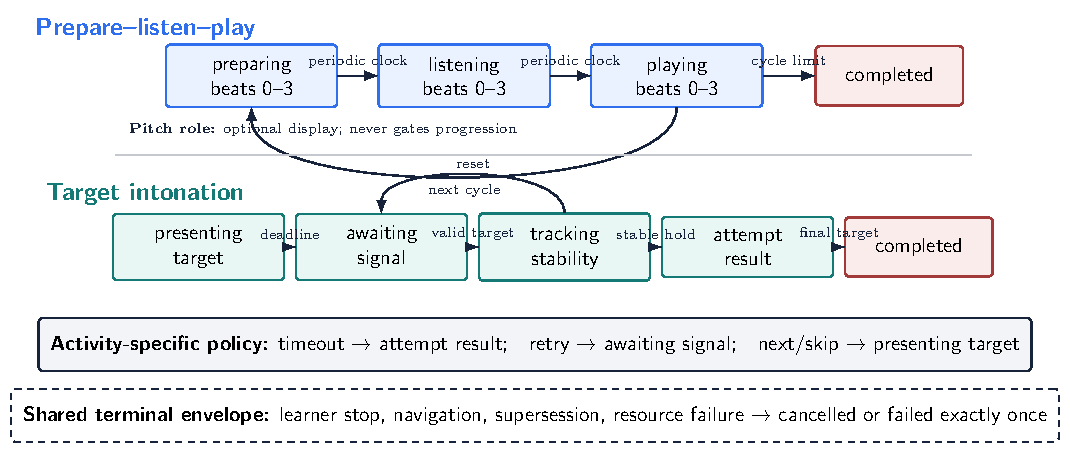
\includegraphics[width=\textwidth]{figures/activity-lifecycles.pdf}
\caption{Contrasting transition drivers within the same lifecycle envelope.
PLP advances on periodic clock ticks through a fixed cycle. Target intonation
advances on pitch estimates, one-shot deadlines, and learner commands; invalid,
wrong-note, or discontinuous input resets stability without changing the
shared lifecycle contract.}
\label{fig:lifecycles}
\end{figure}

\subsection{Pure Target-Relative Evaluation}

\texttt{IntonationEvaluator} is a deterministic TypeScript object with no
Angular, Ionic, DOM, Web Audio, persistence, or wall-clock dependency. It
receives a \texttt{NoteTarget}, configuration, and timestamped samples. For a
voiced estimate $f$ it computes
\[
 c = 1200\log_2(f/f_{\mathrm{target}}).
\]
It classifies no signal, invalid estimate, detector-range violation, wrong
note, far flat, flat, within tolerance, sharp, far sharp, and unstable.

Correct note identity is checked against the target sounding MIDI identity
before tuning success is possible. Consequently, a frequency near another
chromatic note cannot be reported as in tune even if it is locally close to
that note. A stable hold additionally requires the configured duration,
minimum estimate count, maximum spread, and maximum signal gap. Silence, a
wrong note, excessive spread, or a long gap resets the window. Timestamps are
injected; exact inclusivity at tolerance, spread, duration, detector-range,
and gap boundaries is covered by tests.

Table~\ref{tab:activities} shows why the two modules are not variants of one
state machine.

\begin{table}[t]
\caption{Activity-specific policy behind the shared lifecycle.}
\label{tab:activities}
\centering
\small
\begin{tabularx}{\textwidth}{@{}p{.22\textwidth}XX@{}}
\toprule
Property & Prepare--listen--play & Target intonation\\
\midrule
Primary driver & Periodic four-beat clock & Pitch events, deadlines, commands\\
Pedagogical unit & Prepare/listen/play cycle & Explicit target and attempt\\
Pitch role & Optional, non-gating display & Target-relative, gating evidence\\
Progress condition & Fixed phase/cycle count & Stable hold, timeout, skip, retry\\
Feedback target & Reference for imitation & Written-to-sounding target identity\\
Timer use & One periodic subscription & Presentation and attempt one-shots\\
Result granularity & Cycles and bounded means & Target attempts and summary metrics\\
\bottomrule
\end{tabularx}
\end{table}

\section{Implementation}\label{sec:implementation}

The application uses Angular~15 and Ionic~7 for its web interface and
Capacitor~6 for Android and iOS packaging. Activity modules, lifecycle/domain
contracts, adapters, and route views reside in separate source directories.
The PLP route and target-intonation route compose the same production clock,
audio, pitch, notation, instrument-registry, and persistence adapters.

The target-intonation defaults are three targets, optional reference playback
enabled, a 1,000-ms presentation, $\pm10$-cent tolerance, 1,500-ms hold,
12-cent maximum spread, four valid estimates, 350-ms maximum gap, 10,000-ms
attempt timeout, and three attempts per target. Detector bounds default to
140--2,000 Hz. These values are explicit configuration and persisted with each
session; they are implementation starting points rather than validated
learning thresholds. Sensitivity is transparent: stricter tolerance or spread
reduces acceptance, longer hold and larger estimate count increase required
evidence, and a shorter gap resets stability more readily.

Controllers are tested with fake ports and injected timestamps. Page tests
verify snapshot-to-view mapping and command dispatch. The chromatic-tuner gauge
is a pure target-relative presenter: it receives display values and owns no
pitch session. Route tests verify launch and exactly-once cancellation when
switching activities.

\section{Technical Evaluation}\label{sec:evaluation}

\subsection{Questions and Method}

The evaluation operationalizes the research question through four technical
questions:
\begin{description}
\item[E1] Do deterministic traces satisfy each activity's transition,
pitch-target, terminal, and ownership semantics?
\item[E2] Are activity-specific dependencies kept outside the bounded shared
core?
\item[E3] How local was the change required to add the second activity after
the PLP migration?
\item[E4] Does the two-activity application continue to compile and compose
across the web, Android, and iOS targets?
\end{description}

E1 uses Jasmine tests with fake clock, pitch, audio, notation, and persistence
ports. E2 uses an executable import-boundary check together with file-level
inspection. E3 treats commit \texttt{45daf1c} (the completed PLP migration) as
the frozen comparison point and classifies every production change through the
second-activity integration commit. Files are classified as new
target-intonation module, shared contract extension, shared adapter reuse, PLP
modification, host/routing/presentation integration, or unrelated correction.
E4 uses clean package installation, linting, production web compilation,
isolated Capacitor synchronization, native builds, and route rendering where
available.

\subsection{Behavioral and Boundary Results}

All 98 automated tests passed. Table~\ref{tab:tests} separates the relevant
evidence rather than treating the aggregate count as coverage. The evaluator
suite checks exact target frequency, positive and negative tolerance
boundaries, flat/sharp and far bands, wrong chromatic notes, transposition,
A4 values of 430, 440, and 450 Hz, silence, invalid/non-finite and
out-of-range input, estimate count, stable duration, spread, gaps, recovery,
and exact thresholds. Controller tests exercise stable success, both timeout
forms, retry, skip, next, multiple targets, maximum attempts, stop,
navigation cancellation, restart, supersession, microphone failure, reference
playback failure, and exactly-once cleanup.

\begin{table}[t]
\caption{Deterministic evidence in the verified 98-test suite.}
\label{tab:tests}
\centering
\small
\begin{tabularx}{\textwidth}{@{}l r X@{}}
\toprule
Evidence group & Tests & Representative verified property\\
\midrule
Intonation evaluator & 20 & Explicit-target cents, note identity, stability resets\\
Intonation controller & 16 & Event transitions, policy, terminal/resource ownership\\
Intonation persistence & 3 & Typed bounded DTO mapping and dispatch\\
Target page/view & 4 & Snapshot mapping and command dispatch\\
Tabs/session routing & 4 & Selection, route launch, supersession cancellation\\
Route definition & 1 & Independent lazy activity launches\\
Tuner additions & 2 & Explicit-target wrong-note behavior and local DOM\\
Existing regression suite & 48 & PLP, music domain, lifecycle, services, views\\
\midrule
Total & 98 & All passed\\
\bottomrule
\end{tabularx}
\end{table}

The dependency-boundary check passed: neither controller imports Angular,
Ionic, Capacitor, Firebase, DOM, or Web Audio APIs, and no activity-specific
branch occurs in the shared lifecycle core. The typed instrument/asset audit
also passed for all three instruments, 110 note definitions, and 189 exact
asset paths, with no missing, duplicate, or traversal-unsafe paths.

\subsection{Change-Surface Results}

From the frozen PLP point to second-activity integration, the production
change comprised six added and 12 modified files, with 2,487 added and 51
deleted lines. Table~\ref{tab:change} gives the category distribution. The
three new activity files contain the evaluator, controller, and types. The
shared lifecycle contract changed by six added lines to expose one-shot time
and target notation; seven shared files were touched overall, primarily to
implement or persist those capabilities. The PLP controller file's SHA-256
remained \texttt{8fcdbe...}, and its controller logic had zero changed lines.

\begin{table}[t]
\caption{Production change surface after the frozen PLP migration point. Line
counts describe modification locality; they are not a measure of design
quality.}
\label{tab:change}
\centering
\small
\begin{tabularx}{\textwidth}{@{}X r r r@{}}
\toprule
Category & Files & Added & Deleted\\
\midrule
New target-intonation module & 3 & 1,297 & 0\\
Shared contract extension & 1 & 6 & 0\\
Shared adapter reuse & 6 & 320 & 21\\
PLP modification & 0 & 0 & 0\\
Host/routing/presentation integration & 8 & 864 & 30\\
Unrelated correction & 0 & 0 & 0\\
\midrule
Total & 18 & 2,487 & 51\\
\bottomrule
\end{tabularx}
\end{table}

The largest integration cost occurred in the new activity-specific UI and
composition, not in the lifecycle. Line counts alone cannot establish
extensibility. Their value here is triangulated with repository history,
unchanged PLP-controller content, passing PLP traces, and the absence of
activity branches in the core. Together, these observations show that the
second pedagogical protocol was introduced by adding a module and extending
two narrow capabilities rather than rewriting the first activity or
generalizing both into one transition engine.

\subsection{Cross-Platform Verification}

Table~\ref{tab:platform} reports the performed build evidence and its boundary.
The web build completed after a clean install, and lint and all tests passed.
Android was synchronized in an isolated copy, compiled as a Java~17 debug
build, and passed its unit-test task. iOS was likewise synchronized in an
isolated copy and compiled unsigned for an iOS simulator with Xcode~26.6. The
app was installed and launched on an iPhone~17 Pro simulator running
iOS~26.5; both activity routes rendered. No Android emulator launch or
physical-device acoustic run was performed.

\begin{table}[t]
\caption{Cross-platform verification performed on the two-activity build.}
\label{tab:platform}
\centering
\small
\begin{tabularx}{\textwidth}{@{}l l X@{}}
\toprule
Target & Result & Verified boundary\\
\midrule
Web & Passed & Clean install, lint, 98 tests, production compilation\\
Android & Passed & Isolated sync, Java~17 debug build, unit-test task\\
iOS & Passed & Isolated sync, unsigned simulator compile, install/launch\\
Routes & Passed on iOS/web & PLP and target-intonation surfaces rendered\\
\bottomrule
\end{tabularx}
\end{table}

\section{Discussion}\label{sec:discussion}

The evaluation supports the central claim: the bounded activity lifecycle and
capability architecture was instantiated by two functionally and temporally
contrasting music-learning activities while preserving the first activity
controller and requiring only minimal shared capability extensions. This
matters because a periodic instructional sequence and a pitch-gated attempt
protocol stress different scheduling, feedback, and termination concerns. The
architecture accommodated both without moving their policies into shared code.

\subsection{Extensibility as Localized Pedagogical Change}

Extensibility here is not inferred from modular naming. It is observed through
a concrete second instantiation. New pedagogical states, commands, feedback,
stability logic, and attempt results are confined to the target-intonation
module. The shared evolution---one-shot time and target notation---represents
capabilities meaningful to more than one potential activity, while persistence
dispatch remains an adapter concern. Unchanged PLP content and traces show that
adding event-driven gating did not alter fixed-cycle semantics.

This locality improves reproducibility and reviewability. A researcher can
inspect the evaluator independently of browser audio, replay controller traces
with timestamps, and determine which code changed for the second protocol.
For maintainers, the lifecycle centralizes cancellation and result envelopes
without requiring a universal state-machine language. For educators and
designers, activity controllers remain a visible expression of pedagogical
sequence rather than configuration interpreted by a generic engine.

\subsection{Pedagogical Diversity on a Common Musical Domain}

The preserved pedagogical rationale also clarifies why separation is useful.
PLP sequences preparation, imitation, and performance without gating progress
on detected pitch. Target intonation intentionally provides explicit
target-relative feedback and requires stable production. Neither policy is
universally preferable; they support different practice goals. Sharing the
typed written/sounding target allows both activities to agree on musical
identity while disagreeing productively about feedback and progression.

The wrong-note rule is a concrete example. A chromatic tuner normally reports
deviation from the nearest semitone. In a target exercise, that behavior can
reward a stable but unintended note. Binding evaluation to the explicit
sounding target prevents that category error and makes transposition and A4
selection testable parts of the activity contract.

\subsection{Cross-Platform Maintainability}

The adapters keep controllers independent of Angular, Ionic, Capacitor, and
Firebase. This does not make native behavior identical, but it lets the same
deterministic activity evidence run before platform packaging and limits
native verification to composition boundaries. Successful web, Android, and
iOS builds after the second activity provide evidence that the architectural
change did not sacrifice the application's hybrid deployment model.

\section{Limitations and Future Work}\label{sec:limitations}

The evaluation is architectural, not educational. No claim is made about
learning gains, usability, engagement, or the pedagogical optimality of the
default intonation thresholds. Such questions require separate participant
studies and are outside this manuscript.

The pitch evaluator is verified with deterministic estimates rather than
physical microphone input. We did not measure end-to-end detector accuracy,
acquisition latency, audible reference timing, or the acoustic correctness of
recorded reference tones on devices. Controlled synthetic-signal and physical
instrument experiments should characterize these boundaries before metrics
are interpreted as performance measurements.

The architecture has been demonstrated through two activities within one
application and three wind-instrument definitions. This is stronger evidence
than a single reference implementation but does not establish suitability for
arbitrary activities or musical traditions. A third activity with a different
resource profile, external replication by another developer, and versioned
artifact studies would test transfer further. The current contribution is an
extensible application architecture; packaging a general-purpose toolkit or
framework would require a separately evaluated distribution, public extension
contract, documentation, and independent adopters.

Platform evidence is also asymmetric: iOS route rendering was observed in a
simulator, whereas Android evidence is limited to sync, build, and unit tasks.
Future validation should execute both activities with microphone and audio on
representative physical Android and iOS devices, characterize interruptions,
and evaluate accessibility with users rather than infer it from interface
structure.

\section{Conclusion}\label{sec:Conclusions}

We evolved a pedagogically grounded music-learning application into an
extensible activity architecture that separates a bounded lifecycle and
reusable capabilities from activity-specific logic. Two contrasting
instantiations exercise the result: fixed-cycle, clock-driven
prepare--listen--play and event-driven target intonation with explicit
written-to-sounding pitch semantics and stable-hold evidence.

The second activity was added as its own controller, evaluator, types, and
view. It required a six-line shared contract extension, introduced no
activity-specific branches in the shared core, left the PLP controller
unchanged, and preserved its deterministic trace. Ninety-eight passing tests,
boundary and asset audits, repository-history analysis, and web/Android/iOS
build verification provide convergent evidence for modification locality,
resource ownership, reproducibility, and cross-platform maintainability.

The result offers a defensible basis for adding and studying further
music-learning protocols without collapsing their pedagogical differences.
Future work should complement this architectural evidence with controlled
acoustic characterization, physical-device evaluation, additional
instantiations, and separate studies of educational effectiveness.

\begin{thebibliography}{71}
\sloppy
\raggedright

\bibitem{AcquilinoISMIR}
Acquilino, A., Puranik, N., Fujinaga, I., Scavone, G.: A Dataset and Baseline for Automated Assessment of Timbre Quality in Trumpet Sound. In: Proceedings of the 24th International Society of Music Information Retrieval Conference, pp. 684--691 (2023)

\bibitem{AcquilinoSMAC}
Acquilino, A., Puranik, N., Fujinaga, I., Scavone, G.: Detecting Efficiency in Trumpet Sound Production: Proposed Methodology and Pedagogical Implications. In: Proceedings of the 5th Stockholm Music Acoustic Conference, pp. 72--79. KTH Royal Institute of Technology, Stockholm (2023)

\bibitem{Acquilino22}
Acquilino, A., Scavone, G.: Current State and Future Directions of Technologies for Music Instrument Pedagogy. Frontiers in Psychology \textbf{13} (2022). \url{https://doi.org/10.3389/fpsyg.2022.835609}

\bibitem{AdamsWebber99}
Adams-Webber, J.: Self-reflection in adolescence. Journal of Constructivist Psychology \textbf{12}(3), 203--213 (1999). \url{https://doi.org/10.1080/107205399266073}

\bibitem{Allingham23}
Allingham, E., Wöllner, C.: Putting Practice under the Microscope: The Perceived Uses and Limitations of Slow Instrumental Music Practice. Psychology of Music \textbf{51}(3), 906--923 (2023)

\bibitem{Arban82}
Arban, J.-B.: Arban's Complete Conservatory Method for Trumpet (Cornet): or E-flat Alto, B-flat Tenor, Baritone, Euphonium and B-flat Bass in Treble Clef. Carl Fischer, New York, N.Y. (1982)

\bibitem{Bagga19}
Bagga, S., Maurer, B., Miller, T., Quinlan, L., Silvestri, L., Wells, D., Winqvist, R., Zolotas, M., Demiris, Y.: instruMentor: An Interactive Robot for Musical Instrument Tutoring. In: Proceedings of the 20th Annual Conference on Towards Autonomous Robotic Systems, pp. 303--315 (2019)

\bibitem{Bandiera16}
Bandiera, G., Romani Picas, O., Tokuda, H., Hariya, W., Oishi, K., Serra, X.: Good-sounds.org: A Framework to Explore Goodness in Instrumental Sounds. In: Proceedings of the 17th International Society for Music Information Retrieval Conference (ISMIR), pp. 414--419 (2016)

\bibitem{Bass21}
Bass, L., Clements, P., Kazman, R.: Software Architecture in Practice. 4th edn. Addison-Wesley Professional (2021)

\bibitem{Bauer20}
Bauer, W. I.: Music Learning Today: Digital Pedagogy for Creating, Performing, and Responding to Music. 2nd edn. Oxford University Press, New York, NY (2020)

\bibitem{Bengtsson04}
Bengtsson, P., Lassing, N., Bosch, J., van Vliet, H.: Architecture-level modifiability analysis (ALMA). Journal of Systems and Software \textbf{69}(1--2), 129--147 (2004). \url{https://doi.org/10.1016/S0164-1212(03)00080-3}

\bibitem{Blanco21}
Blanco, A. D., Tassani, S., Ramirez, R.: Real-Time Sound and Motion Feedback for Violin Bow Technique Learning: A Controlled, Randomized Trial. Frontiers in Psychology \textbf{12} (2021). \url{https://doi.org/10.3389/fpsyg.2021.648479}

\bibitem{Bonstrup20}
Bönstrup, M., Iturrate, I., Hebart, M. N., Censor, N., Cohen, L. G.: Mechanisms of Offline Motor Learning at a Microscale of Seconds in Large-Scale Crowdsourced Data. Npj Science of Learning \textbf{5}(1) (2020). \url{https://doi.org/10.1038/s41539-020-0066-9}

\bibitem{Booth09}
Booth, E.: The Music Teaching Artist's Bible: Becoming a Virtuoso Educator. Oxford University Press, Oxford (2009)

\bibitem{Brennan16}
Brennan, J.: Poper's Game: A 21st Century Approach to Addressing Initial Attacks in Practice. International Trumpet Guild Journal \textbf{41}(1), 68--71 (2016)

\bibitem{Brown13}
Brown, R. M., Palmer, C.: Auditory and motor imagery modulate learning in music performance. Frontiers in Human Neuroscience \textbf{7}(320) (2013). \url{https://doi.org/10.3389/fnhum.2013.00320}

\bibitem{Carter16}
Carter, C. E., Grahn, J. A.: Optimizing Music Learning: Exploring How Blocked and Interleaved Practice Schedules Affect Advanced Performance. Frontiers in Psychology \textbf{7} (2016). \url{https://doi.org/10.3389/fpsyg.2016.01251}

\bibitem{Crocco21}
Crocco, L., Meyer, D.: Motor Learning and Teaching Singing: An Overview. Journal of Singing \textbf{77}(5), 693--702 (2021)

\bibitem{Csikszentmihalyi08}
Csikszentmihalyi, M.: Flow: The Psychology of Optimal Experience. 1st Harper Perennial Modern Classics edn. Harper Perennial, New York (2008)

\bibitem{Deterding11}
Deterding, S., Dixon, D., Khaled, R., Nacke, L.: From Game Design Elements to Gamefulness: Defining Gamification. In: Proceedings of the 15th International Academic MindTrek Conference: Envisioning Future Media Environments, pp. 9--15 (2011)

\bibitem{Dewey38}
Dewey, J.: Experience and Education. Kappa Delta Pi, New York (1938)

\bibitem{Dolmage17}
Dolmage, J.: Academic Ableism: Disability and Higher Education. University of Michigan Press, Project Muse (2017)

\bibitem{Engel12}
Engel, A., Bangert, M., Horbank, D., Hijmans, B. S., Wilkens, K., Keller, P. E., Keysers, C.: Learning Piano Melodies in Visuo-Motor or Audio-Motor Training Conditions and the Neural Correlates of Their Cross-Modal Transfer. NeuroImage \textbf{63}(2), 966--978 (2012)

\bibitem{Fleming92}
Fleming, N., Mills, C.: Not Another Inventory, Rather a Catalyst for Reflection. To Improve the Academy \textbf{11}(1), 137--155 (1992)

\bibitem{Fleming06}
Fleming, N., Baume, D.: Learning Styles Again: VARKing up the Right Tree! Educational Developments, SEDA Ltd \textbf{7}(4), 4--7 (2006)

\bibitem{Gates21}
Gates, S.: Developing Musical Imagery Contributions from Pedagogy and Cognitive Science. Music Theory Online \textbf{27}(2) (2021)

\bibitem{Gaunt08}
Gaunt, H.: One-to-One Tuition in a Conservatoire: The Perceptions of Instrumental and Vocal Teachers. Psychology of Music \textbf{36}(2), 215--245 (2008)

\bibitem{Gebel13}
Gebel, B., Braun, C., Kaza, E., Altenmüller, E., Lotze, M.: Instrument-Specific Brain Activation in Sensorimotor and Auditory Representation in Musicians. NeuroImage \textbf{74}, 37--44 (2013)

\bibitem{Guadagnoli01}
Guadagnoli, M. A., Kohl, R. M.: Knowledge of Results for Motor Learning: Relationship between Error Estimation and Knowledge of Results Frequency. Journal of Motor Behavior \textbf{33}(2), 217--224 (2001)

\bibitem{Guadagnoli04}
Guadagnoli, M. A., Lee, T. D.: Challenge Point: A Framework for Conceptualizing the Effects of Various Practice Conditions in Motor Learning. Journal of Motor Behavior \textbf{36}(2), 212--224 (2004)

\bibitem{Hagglund96}
Hagglund, K. L., Jacobs, K.: Physical and Mental Practices of Music Students as They Relate to the Occurrence of Music-Related Injuries. Work \textbf{6}, 11--24 (1996)

\bibitem{Halpern04}
Halpern, A. R., Zatorre, R. J., Bouffard, M., Johnson, J. A.: Behavioral and Neural Correlates of Perceived and Imagined Musical Timbre. Neuropsychologia \textbf{42}(9), 1281--1292 (2004)

\bibitem{Harrison14}
Harrison, S. D., O’Bryan, J.: Teaching Singing in the 21st Century. Springer, New York (2014)

\bibitem{Hehir02}
Hehir, T.: Eliminating Ableism in Education. Harvard Educational Review \textbf{72}(1), 1--32 (2002)

\bibitem{Jacobs06}
Jacobs, A., Nelson, B.: Also Sprach Arnold Jacobs: A Developmental Guide for Brass Wind Musicians. Polymnia Press (2006)

\bibitem{Jellison15}
Jellison, J. A.: Including Everyone: Creating Music Classrooms Where All Children Learn. Oxford University Press (2015)

\bibitem{Karakaş24}
Karakaş, B., Dündar, M.: Multi-Sensory Learning in Violin Training. International Journal of Quality in Education \textbf{8}(2), 12--30 (2024)

\bibitem{Katz13}
Katz, J.: The Three Block Model of Universal Design for Learning (UDL): Engaging Students in Inclusive Education. Canadian Journal of Education / Revue Canadienne de L’éducation \textbf{36}(1), 153--194 (2013)

\bibitem{Kohut85}
Kohut, D. L.: Musical Performance: Learning Theory and Pedagogy. Prentice-Hall, Englewood Cliffs, N.J. (1985)

\bibitem{Fiuza22}
Lã, F. M. B., Fiuza, M. B.: Real-Time Visual Feedback in Singing Pedagogy: Current Trends and Future Directions. Applied Sciences \textbf{12}(21), 10781 (2022). \url{https://doi.org/10.3390/app122110781}

\bibitem{Larssen21}
Larssen, B. C., Ho, D. K., Kraeutner, S. N., Hodges, N. J.: Combining Observation and Physical Practice: Benefits of an Interleaved Schedule for Visuomotor Adaptation and Motor Memory Consolidation. Frontiers in Human Neuroscience \textbf{15} (2021). \url{https://doi.org/10.3389/fnhum.2021.614452}

\bibitem{Leman17}
Leman, M., Nijs, L.: Cognition and Technology for Instrumental Music Learning. In: The Routledge Companion to Music, Technology, and Education, pp. 23--35. Routledge (2017)

\bibitem{Lennon12}
Lennon, M., Reed, G.: Instrumental and Vocal Teacher Education: Competences, Roles and Curricula. Music Education Research \textbf{14}(3), 285--308 (2012). \url{https://doi.org/10.1080/14613808.2012.685462}

\bibitem{Li22}
Li, Z., Fan, D., Wang, H., Lu, Z., Liu, C.: Piano Beginner: A Glove-Based Finger Training VR Application. In: Proceedings of the 2022 International Symposium on Control Engineering and Robotics (ISCER), pp. 262--265 (2022)

\bibitem{Maas08}
Maas, E., Robin, D. A., Austermann Hula, S. N., Freedman, S. E., Wulf, G., Ballard, K. J., Schmidt, R. A.: Principles of Motor Learning in Treatment of Motor Speech Disorders. American Journal of Speech-Language Pathology \textbf{17}(3), 277--298 (2008). \url{https://doi.org/10.1044/1058-0360(2008/025)}

\bibitem{Maton09}
Maton, K.: Cumulative and Segmented Learning: Exploring the Role of Curriculum Structures in Knowledge-Building. British Journal of Sociology of Education \textbf{30}(1), 43--57 (2009). \url{https://doi.org/10.1080/01425690802514342}

\bibitem{McCoy04}
McCoy, S. J.: Your Voice, an Inside View: Multimedia Voice Science and Pedagogy. Inside View Press, Princeton, N.J. (2004)

\bibitem{McLeod05}
McLeod, P., Wyvill, G.: A Smarter Way to Find Pitch. In: Proceedings of the International Computer Music Conference, pp. 138--141 (2005)

\bibitem{Nijs13}
Nijs, L., Lesaffre, M., Leman, M.: The Musical Instrument as a Natural Extension of the Musician. In: Music and Its Instruments, pp. 467--484. Editions Delatour France (2013)

\bibitem{Nijs14}
Nijs, L., Leman, M.: Interactive Technologies in the Instrumental Music Classroom: A Longitudinal Study with the Music Paint Machine. Computers \& Education \textbf{73}(2), 40--59 (2014). \url{https://doi.org/10.1016/j.compedu.2013.11.008}

\bibitem{Nijs18}
Nijs, L.: Dalcroze Meets Technology: Integrating Music, Movement, and Visuals with the Music Paint Machine. Music Education Research \textbf{20}(2), 163--183 (2018). \url{https://doi.org/10.1080/14613808.2017.1312323}

\bibitem{Paule17}
Paule-Ruiz, M. P., Álvarez-García, V., Pérez-Pérez, J. R., Álvarez-Sierra, M., Trespalacios-Menéndez, F.: Music Learning in Preschool with Mobile Devices. Behaviour and Information Technology \textbf{36}(1), 95--111 (2017). \url{https://doi.org/10.1080/0144929X.2016.1198421}

\bibitem{Parnas72}
Parnas, D. L.: On the Criteria to Be Used in Decomposing Systems into Modules. Communications of the ACM \textbf{15}(12), 1053--1058 (1972). \url{https://doi.org/10.1145/361598.361623}

\bibitem{Rizzolatti04}
Rizzolatti, G., Craighero, L.: The Mirror-Neuron System. Annual Review of Neuroscience \textbf{27}, 169--192 (2004). \url{https://doi.org/10.1146/annurev.neuro.27.070203.144230}

\bibitem{Robine07}
Robine, M., Percival, G., Lagrange, M.: Analysis of Saxophone Performance for Computer-Assisted Tutoring. In: Proceedings of the 2007 International Computer Music Conference, pp. 381--384. International Computer Music Association, Copenhagen, Denmark (2007)

\bibitem{Romani15}
Romani Picas, O., Parra Rodriguez, H., Dabiri, D., Tokuda, H., Hariya, W., Oishi, K., Serra, X.: A Real-Time System for Measuring Sound Goodness in Instrumental Sounds. In: Proceedings of the 138th Audio Engineering Society Convention, pp. 1--11. Audio Engineering Society (2015)

\bibitem{Schmidt20}
Schmidt, R. A., Lee, T. D.: Motor Learning and Performance: From Principles to Application. 6th edn. Human Kinetics, Champaign, IL (2020)

\bibitem{Shi23}
Shi, Y.: The Use of Mobile Internet Platforms and Applications in Vocal Training: Synergy of Technological and Pedagogical Solutions. Interactive Learning Environments \textbf{31}(6), 3780--3791 (2023). \url{https://doi.org/10.1080/10494820.2021.1943456}

\bibitem{Stambaugh11}
Stambaugh, L. A.: When Repetition Isn’t the Best Practice Strategy: Effects of Blocked and Random Practice Schedules. Journal of Research in Music Education \textbf{58}(4), 368--383 (2011). \url{https://doi.org/10.1177/0022429410385945}

\bibitem{Steen07}
Steenstrup, K.: Teaching Brass. Det Jyske Musikkonservatorium (2007)

\bibitem{Steen17}
Steenstrup, K.: Blow Your Mind. Aarhus University Press (2017)

\bibitem{Steen21}
Steenstrup, K., Haumann, N. T., Kleber, B., Camarasa, C., Vuust, P., Petersen, B.: Imagine, Sing, Play: Combined Mental, Vocal, and Physical Practice Improves Musical Performance. Frontiers in Psychology \textbf{12} (2021). \url{https://doi.org/10.3389/fpsyg.2021.757052}

\bibitem{Steen23}
Steenstrup, K.: Deep Practice, Peak Performance: The Science of Musical Learning. The Royal Academy of Music, Aarhus (2023)

\bibitem{Tullberg22}
Tullberg, M.: Affordances of Musical Instruments: Conceptual Consideration. Frontiers in Psychology \textbf{13} (2022). \url{https://doi.org/10.3389/fpsyg.2022.974820}

\bibitem{Vera08}
Vera, J. G., Alvarez, J. C. B., Medina, M. M.: Effects of Different Practice Conditions on Acquisition, Retention, and Transfer of Soccer Skills by 9-Year-Old Schoolchildren. Perceptual and Motor Skills \textbf{106}(2), 447--460 (2008). \url{https://doi.org/10.2466/pms.106.2.447-460}

\bibitem{Waddell19}
Waddell, G., Williamon, A.: Technology Use and Attitudes in Music Learning. Frontiers in ICT \textbf{6} (2019). \url{https://doi.org/10.3389/fict.2019.00011}

\bibitem{Webster12}
Webster, P. R.: Key Research in Music Technology and Music Teaching and Learning. Journal of Music, Technology and Education \textbf{4}(2--3), 115--130 (2012). \url{https://doi.org/10.1386/jmte.4.2-3.115\_1}

\bibitem{Weisberg07}
Weisberg, A.: The Art of Wind Playing. Meredith Music Publications, Galesville, MD, and Milwaukee, WI (2007)

\bibitem{Welch05}
Welch, G. F., Howard, D. M., Himonides, E., Brereton, J. S.: Real-Time Feedback in the Singing Studio: An Innovatory Action-Research Project Using New Voice Technology. Music Education Research \textbf{7}(2), 225--249 (2005). \url{https://doi.org/10.1080/14613800500169779}

\bibitem{Westphal90}
Westphal, F. W.: Guide to Teaching Woodwinds. 5th edn. Brown Publishers, Dubuque, IA (1990)

\bibitem{Yin05}
Yin, J., Wang, Y., Hsu, D.: Digital Violin Tutor: An Integrated System for Beginning Violin Learners. In: MULTIMEDIA '05: Proceedings of the 13th Annual ACM International Conference on Multimedia, pp. 976--985 (2005). \url{https://doi.org/10.1145/1101149.1101353}

\bibitem{Zatorre05}
Zatorre, R. J., Halpern, A. R.: Mental Concerts: Musical Imagery and Auditory Cortex. Neuron \textbf{47}, 9--12 (2005). \url{https://doi.org/10.1016/j.neuron.2005.06.013}

\end{thebibliography}
\end{document}
